\input{../Preambulos/preambulo_materiales}

\title{\vspace{-2cm} Lista de ejercicios a cuenta \\ {\large Curso Física Computacional} \vspace{-3ex}}
\author{M. en C. Gustavo Contreras Mayén. \texttt{gux7avo@ciencias.unam.mx}}
\date{}

\begin{document}

\fontsize{14}{14}\selectfont
\vspace{-4cm}
\maketitle


\section{Tema 1.}


\section{Tema 2.}

\subsection{Diferenciación.}

\begin{enumerate}
\item Demuestra que la aproximación a la derivada por diferencias hacia adelante de orden $\order{h^{2}}$ es:
\begin{align*}
\pderivada{f} (x) = \dfrac{- 3 f (x) \, + 4 \, f (x + h) - f (x + 2 \, h)}{2 \, h}
\end{align*}
\item Demuestra que a la derivada por diferencias hacia atrás de orden $\order{h^{2}}$ es::
\begin{align*}
\pderivada{f} (x) = \dfrac{3 \, f (x) \, - 4 \, f (x + h) + f (x + 2 \, h)}{2 \, h}
\end{align*}
\item Del ejercicio del mecanismo articulado, obtener las tres gráficas:
\begin{enumerate}[label=\roman*)]
\item Puntos de velocidad angular $\dot{\beta}$ de la tabla.
\item Nuevos puntos interpolados, ocupando interpolación de Lagrange, Newton o del módulo \texttt{numpy} o \texttt{scipy}.
\item Una curva de interpolación con \texttt{scipy}.
\end{enumerate}
\begin{figure}[H]
    \centering
    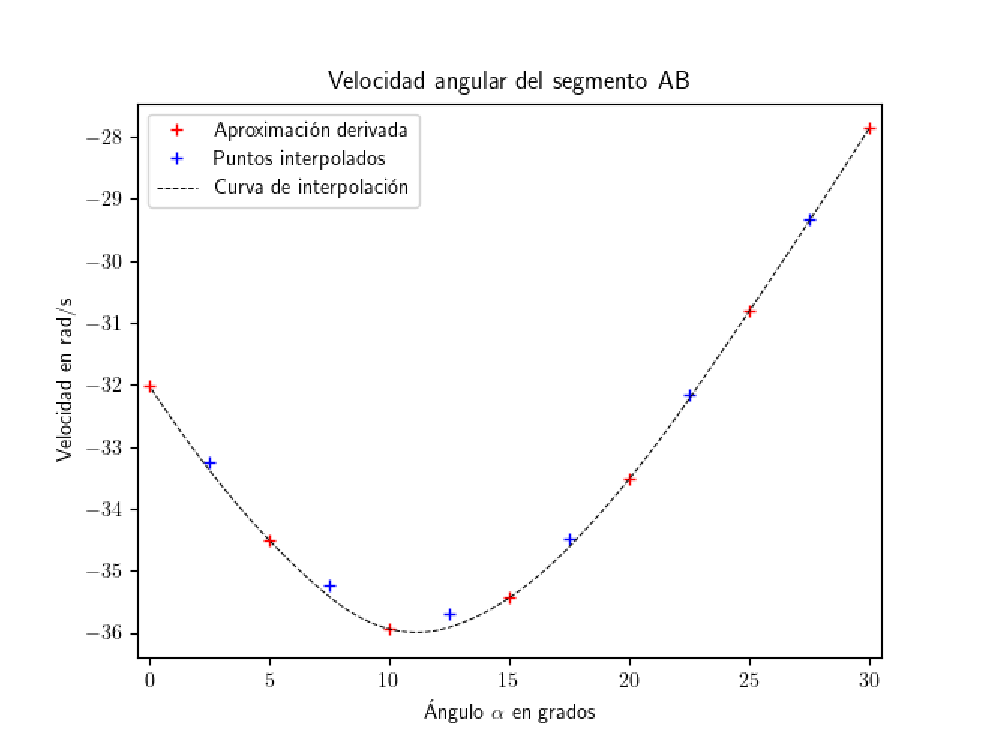
\includegraphics[scale=0.55]{Imagenes/diferenciacion_ejercicio_segmento_03.eps}
    \caption{Esta sería la tercera gráfica que conjunta los tres puntos pedidos del ejercicio de los segmentos articulados.}
\end{figure}
\item Del ejercicio del circuito $RL$, obtener las tres gráficas:
\begin{enumerate}[label=\roman*)]
\item Voltajes para los tiempos indicados en la tabla.
\item Nuevos puntos interpolados, ocupando interpolación de Lagrange, Newton o del módulo \texttt{numpy} o \texttt{scipy}.
\item Una curva de interpolación con \texttt{scipy}.
\end{enumerate}
\begin{figure}
    \centering
    \includegraphics[scale=0.55]{Imagenes/diferenciacion_ejercicio_RL_03.png}
    \caption{Esta sería la tercera gráfica que conjunta los tres puntos pedidos para el ejercicio del circuito $RL$.}
\end{figure}

\end{enumerate}


\end{document}